%%%%%%%%%%%%%%%%%%%%%%%%%%%%%%%%%%%%%%%%%
% Arsclassica Article
% Structure Specification File
%
% This file has been downloaded from:
% http://www.LaTeXTemplates.com
%
% Original author:
% Lorenzo Pantieri (http://www.lorenzopantieri.net) with extensive modifications by:
% Vel (vel@latextemplates.com)
%
% License:
% CC BY-NC-SA 3.0 (http://creativecommons.org/licenses/by-nc-sa/3.0/)
%
%%%%%%%%%%%%%%%%%%%%%%%%%%%%%%%%%%%%%%%%%

%----------------------------------------------------------------------------------------
%	REQUIRED PACKAGES
%----------------------------------------------------------------------------------------

\usepackage[
nochapters, % Turn off chapters since this is an article        
beramono, % Use the Bera Mono font for monospaced text (\texttt)
eulermath,% Use the Euler font for mathematics
pdfspacing, % Makes use of pdftex’ letter spacing capabilities via the microtype package
dottedtoc % Dotted lines leading to the page numbers in the table of contents
]{classicthesis} % The layout is based on the Classic Thesis style

\usepackage{url} % Allows usage of hyperlinks
\usepackage{tabularx}
\usepackage{arsclassica} % Modifies the Classic Thesis package
\usepackage[T1]{fontenc} % Use 8-bit encoding that has 256 glyphs
\usepackage[utf8]{inputenc} % Required for including letters with accents
\usepackage[swedish, english]{babel}
\usepackage{graphicx} % Required for including images
\usepackage{enumitem} % Required for manipulating the whitespace between and within lists
\usepackage{lipsum} % Used for inserting dummy 'Lorem ipsum' text into the template
\usepackage{subfig} % Required for creating figures with multiple parts (subfigures)
\usepackage{amsmath,amssymb,amsthm} % For including math equations, theorems, symbols, etc
\usepackage{varioref} % More descriptive referencing

\usepackage{xcolor}
\usepackage{listings}

\definecolor{mGreen}{rgb}{0,0.6,0}
\definecolor{mGray}{rgb}{0.5,0.5,0.5}
\definecolor{mPurple}{rgb}{0.58,0,0.82}
\definecolor{backgroundColour}{rgb}{0.95,0.95,0.92}

\lstdefinestyle{CStyle}{
    backgroundcolor=\color{backgroundColour},   
    commentstyle=\color{mGreen},
    keywordstyle=\color{magenta},
    numberstyle=\tiny\color{mGray},
    stringstyle=\color{mPurple},
    basicstyle=\footnotesize,
    breakatwhitespace=false,         
    breaklines=true,                 
    captionpos=b,                    
    keepspaces=true,                 
    numbers=left,                    
    numbersep=5pt,                  
    showspaces=false,                
    showstringspaces=false,
    showtabs=false,                  
    tabsize=2,
    language=C
}

\usepackage[pages=some, scale=1, angle=0, opacity=0.7]{background}
\backgroundsetup{
  contents={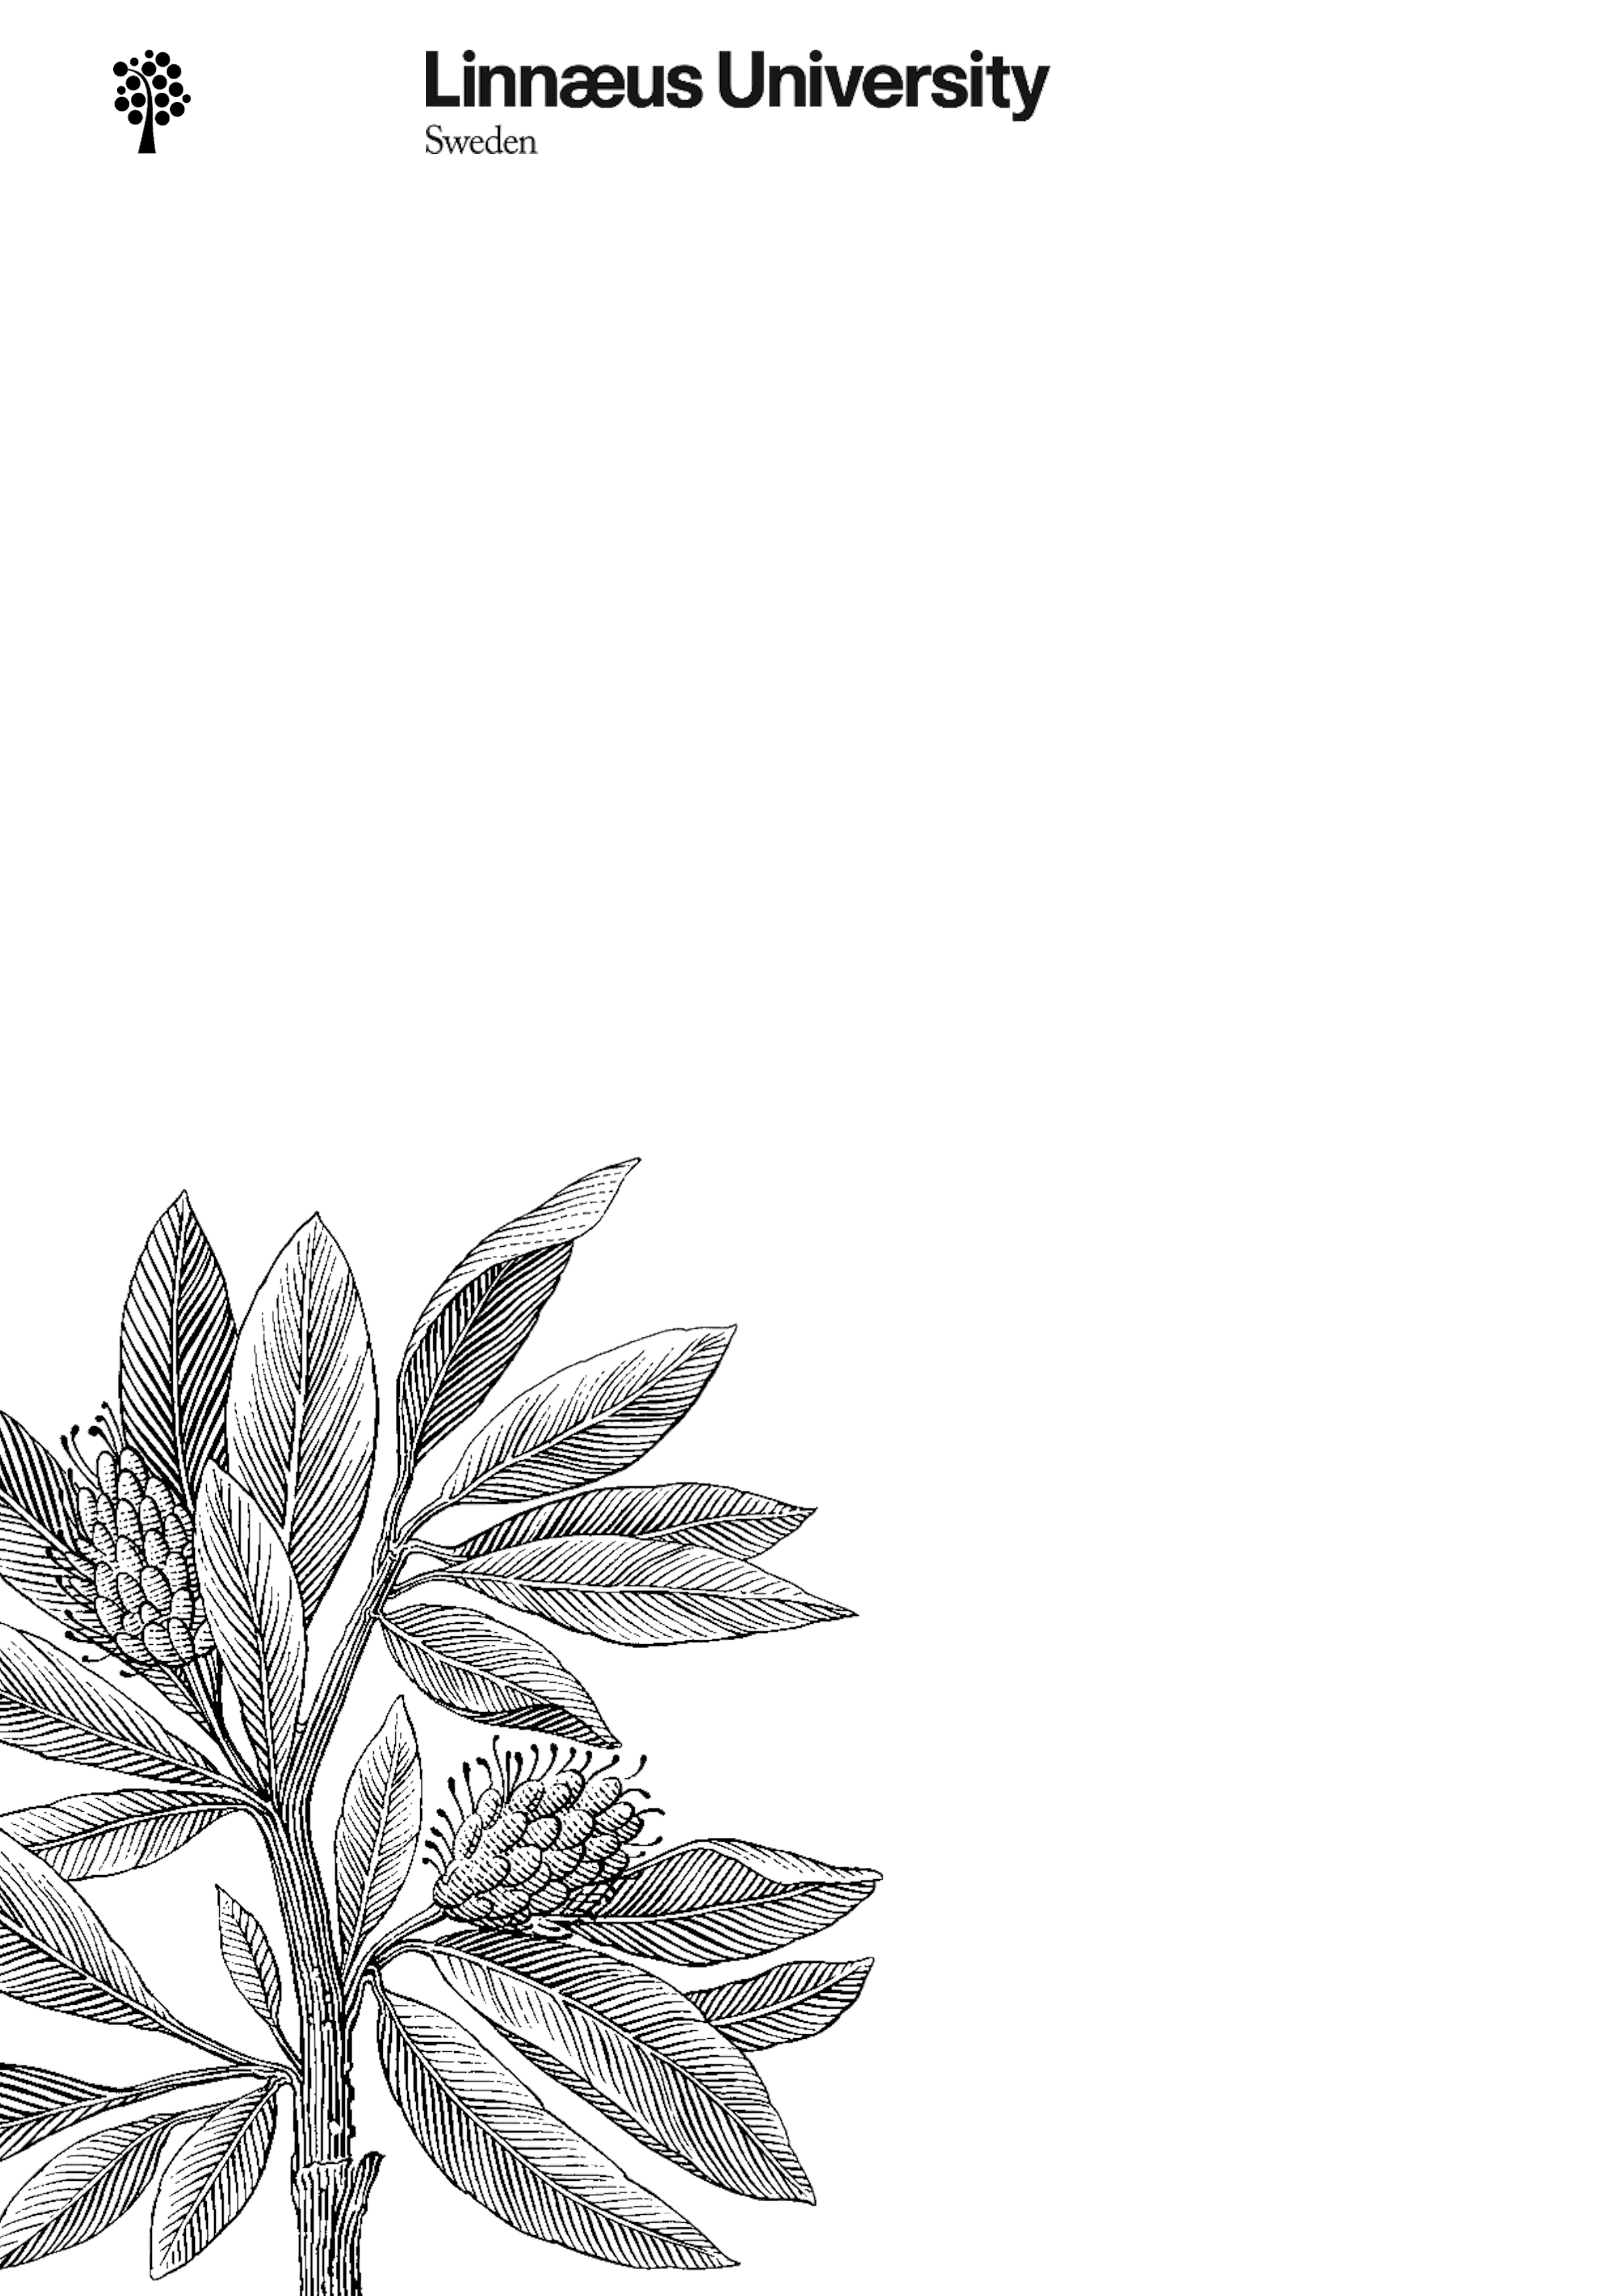
\includegraphics{titlepage_background}}
}
\usepackage{xcolor}

\usepackage{geometry}

\graphicspath{{logo/},{figures/}} % Set the default folder for images
%----------------------------------------------------------------------------------------
%	THEOREM STYLES
%---------------------------------------------------------------------------------------

\theoremstyle{definition} % Define theorem styles here based on the definition style (used for definitions and examples)
\newtheorem{definition}{Definition}

\theoremstyle{plain} % Define theorem styles here based on the plain style (used for theorems, lemmas, propositions)
\newtheorem{theorem}{Theorem}

\theoremstyle{remark} % Define theorem styles here based on the remark style (used for remarks and notes)

%----------------------------------------------------------------------------------------
%	HYPERLINKS
%---------------------------------------------------------------------------------------

\hypersetup{
%draft, % Uncomment to remove all links (useful for printing in black and white)
colorlinks=true, breaklinks=true, bookmarks=true,bookmarksnumbered,
urlcolor=webbrown, linkcolor=RoyalBlue, citecolor=webgreen, % Link colors
pdftitle={}, % PDF title
pdfauthor={\textcopyright}, % PDF Author
pdfsubject={}, % PDF Subject
pdfkeywords={}, % PDF Keywords
pdfcreator={pdfLaTeX}, % PDF Creator
pdfproducer={LaTeX with hyperref and ClassicThesis} % PDF producer
}



\newcommand*{\reporttitle}[1]{\def\rtitle{\normalfont\spacedallcaps #1}}
\newcommand*{\reportsubtitle}[1]{\def\rsubtitle{#1}}
\newcommand*{\documenttype}[1]{\def\doctype{#1}}
\newcommand*{\professor}[1]{\def\profname{#1}}
\newcommand*{\authors}[1]{\def\authorsname{\normalfont\spacedallcaps #1}}
\newcommand*{\email}[1]{\def\authorsemail{#1}}
\newcommand*{\authorssecond}[1]{\def\authorssecondname{\normalfont\spacedallcaps #1}}
\newcommand*{\emailsecond}[1]{\def\authorssecondemail{#1}}
\newcommand*{\coursename}[1]{\def\course{#1}}
\newcommand*{\coursecode}[1]{\def\coursecod{\texttt{#1}}}
\newcommand*{\semester}[1]{\def\sem{\texttt{#1}}}